\section{Exact three-dimensional Fable--Erd\H{o}s--Straus transport}
\label{sec:fable-es-tetrahedron}

The canonical project reader contains a four-dimensional raw-cell carrier and
an exact linear transport to the Erd\H{o}s--Straus-aligned Lorentz coordinates
\((T,X,Y,W)\) \cite[Theorem on the exact spatial quarter altitude of the
transported raw-cell tetrahedron]{ESReader}.  The following coordinate
statement is reproduced here because it is the three-dimensional geometry
actually used by the present bridge.

\begin{theorem}[Tetrahedron transport]
\label{thm:transported-raw-tetrahedron}
In the ordered raw-cell basis
\((E_{11},E_{12},E_{21},E_{22})\), put
\[
\begin{aligned}
 v_\ast&=(0,0,1,0)^{\mathsf T},&
 v_0&=(2,2,0,2)^{\mathsf T},\\
 v_+&=(2+\sqrt3,-1,0,2-\sqrt3)^{\mathsf T},&
 v_-&=(2-\sqrt3,-1,0,2+\sqrt3)^{\mathsf T}.
\end{aligned}
\]
The retained raw-cell to Lorentz map is
\begin{equation}
 \Phi_\triangle=
 \begin{pmatrix}
  5/8&0&3/4&5/8\\
  0&1&0&0\\
  3/8&0&5/4&3/8\\
  1/2&0&0&-1/2
 \end{pmatrix},
 \qquad \det\Phi_\triangle=-\frac12.                   \tag{EZ35A}
\end{equation}
It sends these four vertices to
\begin{align}
 z_\ast&=(3/4,0,5/4,0)^{\mathsf T},&
 z_0&=(5/2,2,3/2,0)^{\mathsf T},\nonumber\\
 z_+&=(5/2,-1,3/2,\sqrt3)^{\mathsf T},&
 z_-&=(5/2,-1,3/2,-\sqrt3)^{\mathsf T}.              \tag{EZ35B}
\end{align}
For \(q_{\rm L}(T,X,Y,W)=X^2+Y^2+W^2-T^2\),
\[
 q_{\rm L}(z_\ast)=1,\qquad
 q_{\rm L}(z_0)=q_{\rm L}(z_+)=q_{\rm L}(z_-)=0.       \tag{EZ35C}
\]
After the spatial projection
\(\pi_{\rm sp}(T,X,Y,W)=(X,Y,W)\), write
\(p_a=\pi_{\rm sp}(z_a)\).  Then
\begin{equation}
 \frac{p_0+p_++p_-}{3}-p_\ast=(0,1/4,0),               \tag{EZ35D}
\end{equation}
every face edge has length \(2\sqrt3\), every apex edge has length
\(\sqrt{65}/4\), and the Euclidean volume is \(\sqrt3/4\).
\end{theorem}

\begin{proof}
Multiplication of the matrix in EZ35A by the four displayed raw vertices gives
EZ35B, retaining every coordinate and sign.  Substitution in \(q_{\rm L}\)
gives EZ35C.  The spatial vertices are
\[
 p_\ast=(0,5/4,0),\quad p_0=(2,3/2,0),\quad
 p_+=(-1,3/2,\sqrt3),\quad p_-=(-1,3/2,-\sqrt3).
\]
Their face centroid is \((0,3/2,0)\), which proves EZ35D.  Direct squared
distances are \(12\) between distinct face vertices and \(65/16\) from the
apex to each face vertex.  Finally,
\[
 \frac16\left|
 \det\begin{pmatrix}p_0-p_\ast&p_+-p_\ast&p_--p_\ast\end{pmatrix}
 \right|=\frac{\sqrt3}{4}.
\]
These calculations prove the asserted metric data.  They also show why this
tetrahedron is not to be silently replaced by a regular Euclidean one.
\end{proof}

\begin{figure}[htbp]
\centering
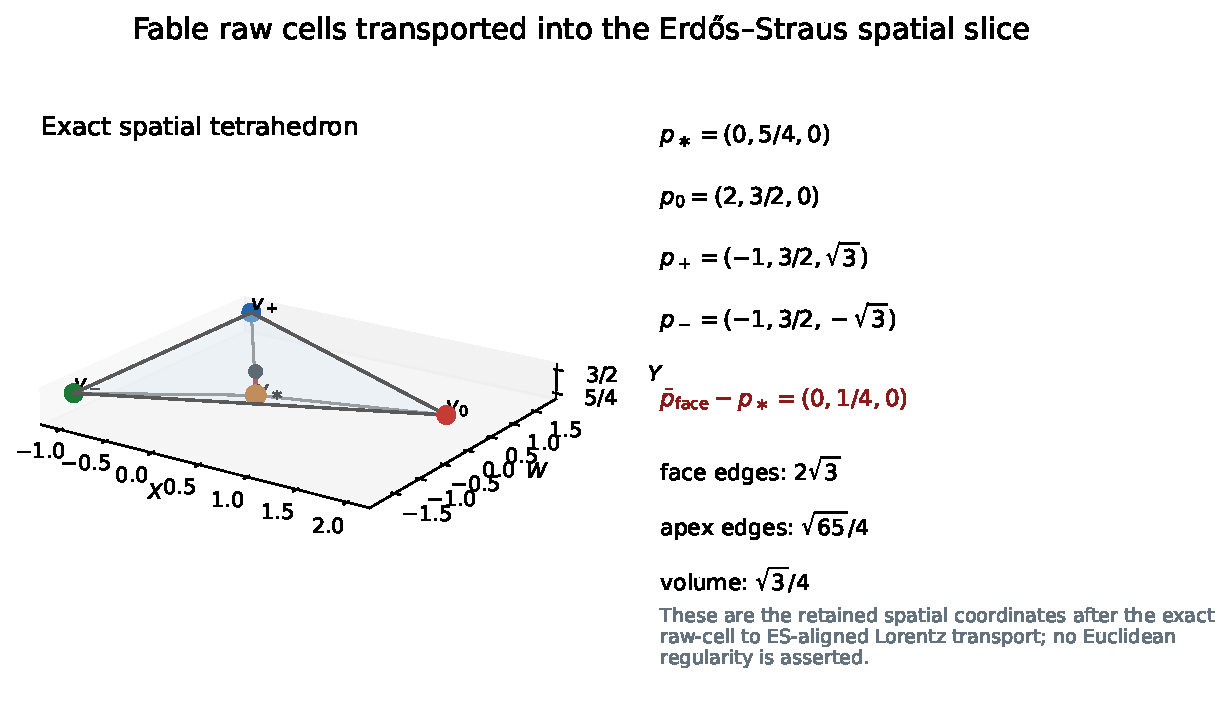
\includegraphics[width=.96\textwidth]{figures/fable-es-raw-tetrahedron-3d.pdf}
\caption{The actual spatial projection in EZ35B--EZ35D.  The three null
vertices lie in the plane \(Y=3/2\); the spacelike apex lies at \(Y=5/4\).
The face centroid and apex have identical \(X,W\) coordinates and differ by
the exact quarter.  Axis coordinates and all metric quantities are retained;
the drawing does not assert Euclidean regularity.  The figure source is
\texttt{tools/generate\_20260920\_illustrations.py}; the exact coordinate
certificate is the local
\texttt{verify\_fable\_es\_raw\_tetrahedron.py}, reproduced from the cited
canonical source calculation.}
\label{fig:fable-es-raw-tetrahedron}
\end{figure}
